%%%%%%%%%%%%%%%%%%%%%%%%%%%%%%%%%%%%%%%%%%%%%%%%%%%%%%%%%%%%%%%%%%%%%%%%%%%%%%%%%%%%%%%%µ%%%%%%%%%%%
%%%  The State of Linked Data - An Extensible Framework to Validate and Build Dataset Profiles  %%%%
%%%%%%%%%%%%%%%%%%%%%%%%%%%%%%%%%%%%%%%%%%%%%%%%%%%%%%%%%%%%%%%%%%%%%%%%%%%%%%%%%%%%%%%%%%%%%%%%%%%%

\documentclass[runningheads,a4paper]{llncs}

\usepackage[utf8]{inputenc}
\usepackage{amssymb}
\setcounter{tocdepth}{3}
\usepackage{graphicx}
\usepackage{tabularx}
\usepackage{url}
\usepackage{listings}
\usepackage{subfigure}
\usepackage{algorithmic}
\usepackage{algorithm}

\graphicspath{ {figures/} }

\newcommand{\keywords}[1]{\par\addvspace\baselineskip
\noindent\keywordname\enspace\ignorespaces#1}

% todo macro
\usepackage{color}
\newtheorem{deflda}{Axiom}
\newcommand{\todo}[1]{\noindent\textcolor{red}{{\bf \{TODO}: #1{\bf \}}}}

% Language Definitions for Turtle
\definecolor{olivegreen}{rgb}{0.2,0.8,0.5}
\definecolor{grey}{rgb}{0.5,0.5,0.5}
\lstdefinelanguage{ttl}{
sensitive=true,
morecomment=[l][\color{brown}]{@},
morecomment=[l][\color{red}]{\#},
morestring=[b][\color{blue}]\",
}

%%%%%%%%%%%%%%%%%%%%%%%%%%%%%%%
%%%  Beginning of document  %%%
%%%%%%%%%%%%%%%%%%%%%%%%%%%%%%%

\begin{document}

% first the title is needed
\title{An Extensible Framework to Validate\\ and Build Dataset Profiles}

\author{Ahmad Assaf\inst{1}\inst{2}, Aline Senart\inst{2} and Rapha\"{e}l Troncy\inst{1} }

\institute{EURECOM, Sophia Antipolis, France. \email{<raphael.troncy@eurecom.fr>}
  \and SAP Labs France. \email{<firstName.lastName@sap.com>}
}

% a short form should be given in case it is too long for the running head
\titlerunning{An Extensible Framework to Validate and Build Dataset Profiles}
%\authorrunning{Assaf, Senart and Troncy}

\maketitle

%%%%%%%%%%%%%%%%%%
%%%  Abstract  %%%
%%%%%%%%%%%%%%%%%%

\begin{abstract}
Linked Open Data (LOD) has emerged as one of the largest collection of interlinked datasets on the web. In order to benefit from this mine of data, one needs to access to descriptive information about each dataset (or metadata). Such metadata information is currently very limited to a few data portals where they are usually provided manually, thus being often incomplete and inconsistent in terms of quality. To address this issue, we propose a scalable automatic approach for extracting, validating and generating descriptive linked dataset profiles. This approach applies several techniques in order to check the validity of the metadata provided and to generate descriptive and statistical information for a particular dataset or for an entire data portal. We experiment with our framework on prominent data portals and we demonstrate that the general state of the Linked Open Data cloud needs more attention as most of the datasets suffer from bad quality metadata and lack some informative metrics.
\keywords{Linked Data, Dataset Profile, Metadata, Data Quality}
\end{abstract}

%%%%%%%%%%%%%%%%%%%%%%%%%
%%%  1. Introduction  %%%
%%%%%%%%%%%%%%%%%%%%%%%%%

\section{Introduction}
\label{sec:introduction}
From 12 datasets cataloged in 2007, the Linked Open Data cloud has grown to nearly 1000 datasets containing more than 82 billion triples\footnote{http://datahub.io/dataset?tags=lod}~\cite{BizerHeath2009}. Data is being published by both the public and private sectors and covers a diverse set of domains from life sciences to media or government data. The Linked Open Data cloud is potentially a gold mine for organizations and individuals who are trying to leverage external data sources in order to produce more informed business decisions~\cite{Boyd2011}. This success lies in the cooperation between data publishers and consumers. Consumers are empowered to find, share and combine information in their applications easily. However, the heterogeneous nature of data sources reflects directly on the data quality as these sources often contain inconsistent as well as misinterpreted and incomplete metadata information. Considering the significant variation in size, the languages used and the freshness of the data, one realized that finding useful datasets without prior knowledge is increasingly complicated. This can be clearly noticed in the LOD Cloud where few datasets such as DBPedia~\cite{Bizer:2009:DCP:1640541.1640848}, Freebase~\cite{Bollacker:2008:FCC:1376616.1376746} and YAGO~\cite{Suchanek:2007:YCS:1242572.1242667} are favored over hidden gems that may include domain specific knowledge more suitable for the tasks at hand.
%Raphael: what are those hidden gems? Give me an example in order to convince me. And for what tasks? Otherwise, this is just speculation

The main entry point for discovering and identifying datasets is either through public data portals such as DataHub\footnote{http://datahub.io} and Europe's Public Data\footnote{http://publicdata.eu} or private search engines such as Quandl\footnote{https://quandl.com/} and Engima\footnote{http://enigma.io/}. Private portals harness manually curated data from various sources and expose them to users either freely or through paid plans. The data available is of higher quality but lesser quantity compared to what is available in public portals. Similarly, in some public data portals, administrators manually review datasets information and attach suitable metadata information. This information is mainly in the form of predefined tags such as \textit{media, geography, life sciences} for organization and clustering purposes. However, the increasing number of datasets available makes the review and curation process unsustainable even when outsourced to communities. Furthermore, the diversity of those datasets makes it harder to classify them in a fixed number of predefined tags that can be subjectively assigned without capturing the essence and breadth of the dataset~\cite{6690016}.

\textit{Data profiling} is the process of creating descriptive information and collet statistics about that data. It is a cardinal activity when facing an unfamiliar dataset~\cite{semwebprofiling}. It helps in assessing the importance of the dataset, in improving users' ability to search and reuse part of the dataset and in detecting irregularities to improve its quality. Data profiling includes typically several tasks:
\begin{itemize}
  \item \textbf{Metadata profiling}: Provides general information on the dataset (dataset description, release and update dates), legal information (license information, openness), practical information (access points, data dumps), etc.
  \item \textbf{Statistical profiling}: Provides statistical information about data types and patterns in the dataset, i.e. properties distribution, number of entities and RDF triples, etc.
  \item \textbf{Topical profiling}: Provides descriptive knowledge on the dataset content and structure. This can be in form of tags and categories used to facilitate search and reuse.
\end{itemize}

In this work, we address the challenges of automatic validation and generation of descriptive datasets profiles. This paper proposes an extensible framework consisting of a processing pipeline that combines techniques for data portals identification, datasets crawling and a set of pluggable modules combining several profiling tasks. The framework validates the provided dataset metadata against an aggregated standard set of information. Metadata fields are automatically corrected when possible, e.g. for adding a missing license reference. Moreover, a report describing the issues that cannot be automatically fixed is created and sent by email to the dataset's maintainer. There exist various statistical and topical profiling tools for both relational and Linked Data. The architecture of the framework allows to easily add them as additional profiling tasks. In this paper, we focus on Linked Data profiling tools as we present our findings on the overall state of Linked Data in some of the prominent data portals.

The remainder of the paper is structured as follows. In Section~\ref{sec:related-work}, we review relevant related work. In Section~\ref{sec:framework}, we describe our proposed framework's architecture and components that validate and generate dataset profiles. In Section~\ref{sec:experiment}, we present the results when running this tool on some of the most prominent data portals and we summarize the main data quality problems. Finally, we conclude and outline some future work in Section~\ref{sec:conclusion}.

%%%%%%%%%%%%%%%%%%%%%%%%%
%%%  2. Related Work  %%%
%%%%%%%%%%%%%%%%%%%%%%%%%

\section{Related Work}
\label{sec:related-work}
There exists a considerable amount of tools that tackle specific profiling tasks. However, to the best of our knowledge, this is the first effort towards extensible automatic assessment and generation of descriptive dataset profiles. For this paper, we will focus on Linked Data profiling tasks. However, one of the advantages of this framework is the ability to easily configure additional profiling tasks accommodating different data types e.g. relational.\\

\textbf{Metadata profiling}: Data Catalog Vocabulary (DCAT) \cite{Erickson:14:DCV} and the Vocabulary of Interlinked Datasets (VoID) \cite{Cyganiak:11:DLD} are concerned with metadata about RDF datasets. There exists several tools aiming at exposing dataset metadata using these vocabularies. In \cite{BoHm:2011:CVD:2030805.2031001} authors generate VoID descriptions limited to a subset of properties that can be automatically deduced from resources within the dataset. However, it still provides data consumers with interesting insights. Quality Assessment of Data Sources (Flemming's Data Quality Assessment Tool)\footnote{http://linkeddata.informatik.hu-berlin.de/LDSrcAss/datenquelle.php} provides basic metadata assessment as it calculates data quality scores based on manual user input. The user should assign weights to the predefined quality metrics and answer a series of questions regarding the dataset. These include, for example, the use of obsolete classes and properties by defining the number of described entities that are assigned disjoint classes, the usage of stable URIs and whether the publisher provides a mailing list for the dataset. The ODI certificate\footnote {https://certificates.theodi.org/} on the other hand provides a description of the published data quality in plain English. It aspires to act as a mark of approval that helps publishers understand how to publish good open data and users how to use it. It gives publishers the ability to provide assurance and support on their data while encouraging further improvements through an ascending scale. ODI comes as an online and free questionnaire for data publishers focusing on certain characteristics about their data. Although these approaches try to perform metadata profiling, they are either incomplete or manual. In our framework, we propose a more automatized and complete approach.\\

\textbf{Statistical profiling}: Calculating statistical information on datasets is vital to applications dealing with query optimization and answering, data cleansing, schema induction and data mining \cite{profilingWebOfData} \cite{datafinland2} \cite{6690016}. Semantic sitemaps \cite{Cyganiak:2008:SSE:1789394.1789457} and RDFStats \cite{Langegger:2009:RER:1674635.1674691} where one of the first to deal with RDF data statistics and summaries. ExpLOD \cite{Khatchadourian:2010:ESE:2155278.2155300} creates statistics on the interlinking between datasets based on \texttt{owl:sameAs} links. In \cite{semwebprofiling} the author introduces a tool that induces the actual schema of the data and gather corresponding statistics accordingly. LODStats  \cite{Auer:2012:LEF:2413941.2413982} is a stream-based approach that calculates more general dataset statistics. ProLOD++ \cite{6816740} is a Web-based tool that allows LOD analysis via automatically computed hierarchical clustering \cite{5452762}. Aether \cite{makela-aether-2014} generates VoID statistical descriptions of RDF datasets. It also provides a Web interface to view and compare VoID descriptions. LODOP \cite{forchhammer_profiles_2014} is a MapReduce framework to compute, optimize and benchmark dataset profiles. The main target for this framework is to optimize the runtime costs for Linked Data profiling. In \cite{DyLDO} authors calculate certain statistical information for the purpose of observing the dynamic changes in datasets.\\

\textbf{Topical Profiling}: Topical and categorical information facilitates dataset search and reuse. Topical profiling focuses on content-wise analysis at the instances and ontological levels. GERBIL \cite{gerbil} is a general entity annotation framework that provides machine processable output allowing efficient querying. In addition, there exist several entity annotation tools and frameworks \cite{Cornolti:2013:FBE:2488388.2488411} but none of those systems are designed specifically for dataset annotation. In \cite{datafinalnd}, authors created a semantic portal to manually annotate and publish metadata about both LOD and non-RDF datasets. In \cite{6690016}, authors automatically assigned Freebase domains to extracted instance labels of some of the LOD Cloud datasets. The goal was to provide automatic domain identification, thus enabling improving datasets clustering and categorization. In \cite{Bohm:2012:LTG:2396761.2398718}, authors extracted dataset topics by exploiting the graph structure and ontological information, thus removing the dependency on textual labels. In  \cite{scalableApproach} authors generate VoID and VoL descriptions via a processing pipeline that extracts dataset topic models ranked on graphical models of selected DBpedia categories.\\

Although the above mentioned tools are able to provide general, statistical and topical information about a dataset, there exist no approach that is able to combine them into a unified profile presented to consumers. Dataset search can be done without relying on attached metadata (tags and categories). For example, there exist several approaches to create LOD indexes. In \cite{Alexander:LDOW09}, authors used VoID descriptions to optimize query processing by determining relevant query-able datasets. In \cite{Harth:2010:DSO:1772690.1772733}, authors created an approximate index structure (QTree) and an algorithm for answering conjunctive queries over Linked Data. SchemEX \cite{Konrath:2012:SEC:2399444.2399563} is a stream-based approach leveraging type and property information of RDF instances to create schema-level indexes.\\
Semantic search engines like Sindice \cite{Delbru2010a}, Swoogle \cite{Ding2004} and Watson \cite{d'Aquin:2011:WMS:2019470.2019476} help in entities lookup but are not designed specifically for dataset search. In \cite{whatShouldILinkTo}, authors utilized the sig.ma index \cite{sig.ma} to identify appropriate data sources for interlinking.

%%%%%%%%%%%%%%%%%%%%%%%%%%%%%%%%%%%
%%%  3. Profiling data portals  %%%
%%%%%%%%%%%%%%%%%%%%%%%%%%%%%%%%%%%

\section{Profiling Data Portals}
\label{sec:framework}

In this section, we provide an overview of the processing steps for validating and generating dataset profiles. Figure 1 shows the main steps which are the following: (i) Data portal identification; (ii) metadata extraction; (iii) instance and resource extraction; (iv) profile validation (v) profiler and report generation.

Our framework is built as a Command Line Interface (CLI) application using Node.js. Related functions are encapsulated into modules that can be easily plugged in/out the processing pipeline. The various steps are explained in details below.

\begin{figure}[h!]
  \centering
    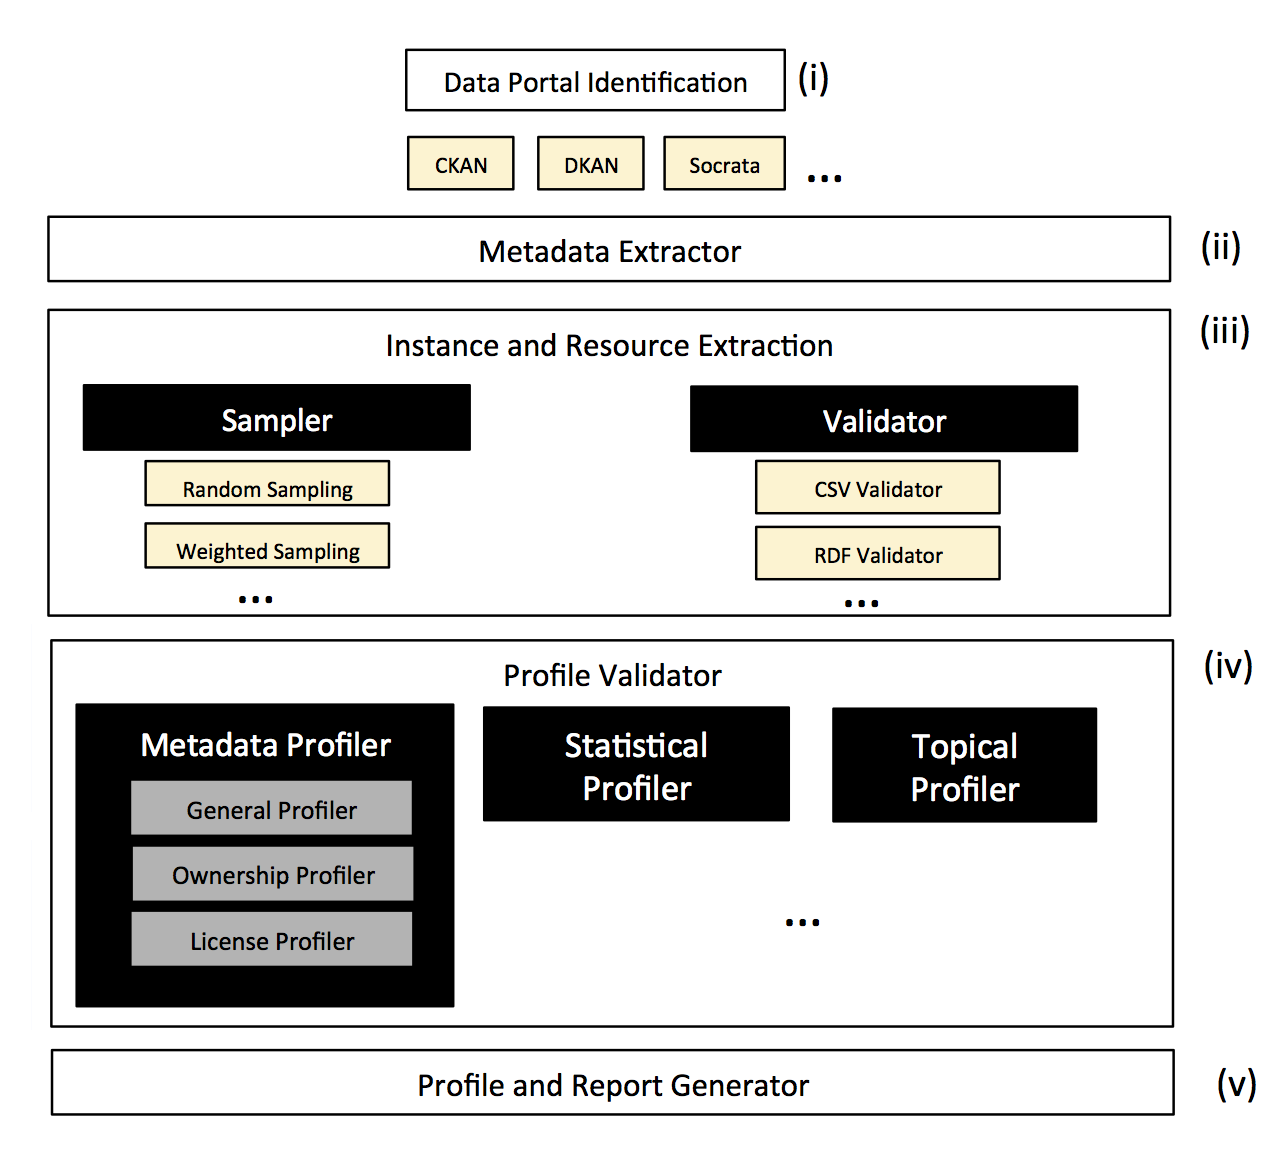
\includegraphics[scale=0.3]{figure-1_architecture.png}
  \caption{Processing pipeline for validating and generating dataset profiles}
\end{figure}

\subsection{Data Portal Identification}

Data portals can be considered as data access points providing tools to facilitate data publishing, sharing, searching and visualization. CKAN\footnote{http://ckan.org} is the world's leading open-source data portal platform powering websites like the DataHub, Europe's Public Data and the U.S Government's open data. Modeled on CKAN, DKAN\footnote{http://drupal.org/project/dkan} is a standalone Drupal distribution that is used in various public data portals as well. Socrata\footnote{http://www.socrata.com} helps public sector organizations improve data-driven decision making by providing a set of solutions including an open data portal. In addition to these tradition data portals, there is a set of tools that allow exposing data directly as RESTful APIs like Datatank\footnote{http://thedatatank.com}, Database-to-API\footnote{https://github.com/project-open-data/db-to-api} and CSV-to-API\footnote{https://github.com/project-open-data/csv-to-api}.\\

Identifying the software powering data portals is a vital first step to understand the API calls structure. Web scraping is a technique for extracting data from Web pages. We rely on several scraping techniques in the identification process which includes a combination of the following:

\begin{itemize}
  \item \textbf{URL inspection}: Check the existence of certain URL patterns. Various CKAN based portals are hosted on subdomains of the \texttt{http://ckan.net}. For example, CKAN Brazil (\texttt{http://br.ckan.net}).
  \item \textbf{Meta tags inspection}: The \texttt{<meta>} tag provides metadata about the HTML document. They are typically used to specify page description, keywords, author, etc. Inspecting the \texttt{content} attribute can indicate the type of the data portal. We use CSS selectors to check the existence of these meta tags. An example of a query selector is \texttt{meta[content*="ckan]} (all meta tags with the attribute content containing the string $CKAN$). This selector can identify CKAN portals whereas the \texttt{meta[content*="Drupal"]} can identify DKAN portals.
  \item \textbf{Document Object Model (DOM) inspection}: Similar to the meta tags inspection, we check the existence of certain DOM elements or properties. For example, CKAN powered portals will have DOM elements with class names like \texttt{ckan-icon} or \texttt{ckan-footer-logo}. A CSS selector like \texttt{.ckan-icon} will be able to check if a DOM element with the class name \texttt{ckan-icon} exists.\\
  The list of elements and properties to inspect is stored in a separate configurable object for each portal. This allows the addition and removal of elements as deemed necessary.
\end{itemize}

The identification process for each portal can be easily customized by overriding the default function. Moreover, adding or removing steps from the identification process can be easily configured.\\
After those preliminary checks, we try to query one of the portal's API endpoints. For example, DataHub is identified as CKAN, so we will query the API endpoint on \texttt{http://datahub.io/api/action/package\_list}. A successful request will list the names of the site's datasets, whereas a failing request will signal a possible failure of the identification process.

\subsection{Metadata Extraction}

Data portals expose a set of information about each dataset as metadata. The model used varies across portals. However, a standard model should contain information about the dataset's title, description, maintainer email, update and creation date, etc. Building a standard metadata model is not the scope of this paper, and since we focus on CKAN-based portals, thus we validate the extracted metadata against the CKAN standard model\footnote{http://demo.ckan.org/api/3/action/package\_show?id=adur\_district\_spending}.  The standard CKAN model contains the following information:\\

\textbf{General information}: General information about the dataset. e.g. title, description, ID, etc. This general information is manually filled by the dataset owner. This information requires manual correction, thus any missing values like the title or description will not be automatically corrected but will appear in the final report. Moreover, we find metadata about the dataset's classification in the portal (groups information) as well as the manually specified tags and keywords. The topical profiler discussed later is able to automatically extract and suggest descriptive tags.\\

\textbf{Access information}: Information about accessing and using the dataset. This includes the dataset URL, license information i.e. license title and URL and information about the dataset's resources. Each resource has as well a set of attached metadata e.g. resource name, URL, format, size, etc.

\textbf{Ownership information}: Information about the ownership of the dataset. e.g. organization details, maintainer details, author, etc.\\ The existence of this information is important to identify the authority on which the generated report and the newly corrected profile will be sent to.\\

\textbf{Provenance information}: Temporal and historical information on the dataset and its resources. For example, creation and update dates, version information, version, etc. Most of this information can be automatically filled and tracked.\\

After identifying the underlying portal software, we perform iterative queries to the API in order to fetch datasets metadata and persist them in a file-based cache system.
Depending on the portal software we can issue specific extraction jobs. For example, in CKAN based portals, we are able to crawl and extract the metadata of a specific dataset, all the datasets in a specific group e.g. LOD Cloud or all the datasets in the portal.\\The caching process can replicate the portal's structure reflecting the various groups or hierarchies defined. Overwriting or disabling caching can be easily done by overloading the call to the extractor.

\subsection{Instance and Resource Extraction}

From the extracted metadata we are able to identify all the resources associated with that dataset. They can have various types like a SPARQL endpoint, API, file, visualization ,etc. However, before extracting the resource instance(s) we perform the following steps:

\begin{itemize}
  \item \textbf{Resource metadata validation and enrichment}: Check the resource attached metadata values. Similar to the dataset metadata, each resource should include information about its mimetype, name, description, format, valid de-referenceable URL, size, type and provenance. The validation process automatically fills up various missing information when possible, like the mimetype and size. However, missing fields like name and description that needs manual input are marked as missing and will appear in the generated summary report.
  \item \textbf{Format validation}: Validate specific resource formats against a linter or a validator. For example, node-csv\footnote{https://github.com/wdavidw/node-csv} for CSV files and n3\footnote{https://github.com/RubenVerborgh/N3.js} to validate N3 and Turtle RDF serializations.
\end{itemize}

Considering that certain dataset contains large amounts of resources and the limited computation power of some machines on which the framework might run on, a sampler module is introduced to execute various sample-based strategies. The following strategies implemented in \cite{scalableApproach} were found to generate accurate results even with comparably small sample size of 10\%.
\begin{itemize}
  \item \textbf{Random Sampling}: Randomly selects resources instances.
  \item \textbf{Weighted Sampling}: Weighs each resources as the ratio of the number of datatype properties used to define a resource over the maximum number of datatype properties over all the datasets resources.
  \item \textbf{Resource Centrality Sampling}: Weighs each resource as the ration of the number of resource types used to describe a particular resource divided by the total number of resource types in the dataset. This is specific and important to RDF datasets where important concepts tend to be more structured and linked to other concepts.
\end{itemize}

However, the sampler is not restricted only to these strategies. Strategies like those introduced in \cite{Leskovec:2006:SLG:1150402.1150479} can be configured and applied in the processing pipeline.

\subsection{Profile Validation}

A dataset profile should include descriptive information about the data examined. In our framework, we have identified three main profiling information. However, the extensibility of our framework allows for additional profiling techniques to be plugged in easily i.e. a quality profiling module reflecting the dataset quality.\\
The implemented profiling tasks are:\\

\textbf{Metadata profiling}\\

The validation process identifies missing information and the ability to automatically correct them. Each set of metadata (general, access, ownership and provenance) is validated and corrected automatically when possible. Each profiler task has a set of metadata fields to check against. The validation process check if each field is defined and if the value assigned is valid.

There exist a bunch of special validation steps for various fields. For example, for ownership information where the maintainer email has to be defined, the validator checks if the email field is an actual valid email address. A similar process is done to URLs whenever found. However, we also issue an HTTP \texttt{HEAD} request in order to check if that URL is reachable or not. For the dataset resources, we use the \texttt{content-header} information when the request is successfull in order to extract, compare and correct further metadata values like mimetype and content size.

Despite the legal issues surrounding Linked Data licenses \cite{nomoneyLOD}, it is still considered a gold mine for organizations who are trying to leverage external data sources in order to produce more informed business decisions \cite{Boyd2011}. In \cite{mckinseyreport} the authors see the potential economic effect unfolding in education, transportation, consumer products, electricity, oil and gas, health care and consumer finance. They estimate the potential annual value enabled by Open Data in these domains to be 3 trillion US Dollars across seven domains. As a result, validating license related information is vital. However, from our experiments, we found out that datasets' license information is noisy. The license names if found are not standardized. For example, Creative Commons CCZero can be also CC0 or CCZero. Moreover,the license URI if found and if de-referenceable can point to different reference knowledge bases e.g. \texttt{http://opendefinition.org}. To overcome this issue, we have manually created a mapping file standardizing the set of possible license names and the reference knowledge base. In addition, we have also used the open source and knowledge license information\footnote{https://github.com/okfn/licenses} to normalize the license information and add extra metadata like the domain, maintainer and open data conformance. \\


\textbf{Statistical profiling}\\

There exist a set of tools designed specifically to provide statistical information about a dataset (see section 2). Providing comprehensive statistical information about a dataset isn't in the scope of this paper. However, to show the extensibility of our framework we provide a simple RDF statistical profiler module that can be easily extended and configured. The information provided for each class is the number: triples, distinct objects, distinct literals, distinct IRI reference objects, distinct blank nodes objects, distinct subjects, distinct IRI reference subjects and distinct blank nodes subjects.\\

\textbf{Topical profiling}\\

Similar to the statistical profiler, a detailed survey of the existing tools can be found in the related work section. However, we implement a very basic topical profiler by applying Named Entity Disambiguation (NED) on the textual description and title of a dataset using DBpedia Spotlight \cite{Mendes:2011:DSS:2063518.2063519}.

\subsection{Profile and Report Generation}

The validation process highlights the missing information and presents them in a human readable report. The report can be automatically sent to the dataset maintainer email if exists in the metadata. The generated report looks like:

\lstset{basicstyle=\scriptsize, backgroundcolor=\color{white}, frame=single, caption={Excerpt of a generated validation report}, label=fresnel, captionpos=b}
\begin{lstlisting}
=======================================================================
                              Metadata Report
=======================================================================
private field exists but there is no value defined
isopen field exists but there is no value defined
group information is missing. Check organization information !
is_organization field exists but there is no value defined
The organization image_url defined for this dataset is not reachable !
=======================================================================
                              Tag Statistics
=======================================================================
There is a total of: 21 [undefined] vocabulary_id fields  100.00%
=======================================================================
                              License Report
=======================================================================
license_title information is missing for this dataset
license_id information is missing for this dataset
License information has been normalized !
=======================================================================
                              License Statistics
=======================================================================
There is one [missing] license_title field  100.00%
There is one [missing] license_id field  100.00%
=======================================================================
                              Resource Statistics
=======================================================================
There is a total of: 10 [missing] url-type fields  100.00%
There is a total of: 9 [missing] created fields  90.00%
There is a total of: 10 [undefined] cache_last_updated fields  100.00%
There is a total of: 10 [undefined] webstore_last_updated fields  100.00%
There is a total of: 10 [undefined] size fields  100.00%
There is a total of: 10 [undefined] hash fields  100.00%
There is a total of: 10 [undefined] mimetype_inner fields  100.00%
There is a total of: 7 [undefined] mimetype fields  70.00%
There is a total of: 10 [undefined] cache_url fields  100.00%
There is a total of: 6 [undefined] name fields  60.00%
There is a total of: 9 [undefined] webstore_url fields  90.00%
There is a total of: 9 [undefined] last_modified fields  90.00%
There is a total of: 10 [undefined] position fields  100.00%
There is one [undefined] format field  10.00%
=======================================================================
                              Resource Connectivity Issues
=======================================================================
There is an access issue with one defined URL:
   - http://dbpedia.org/void/Dataset
\end{lstlisting}

In addition to the generated report, the enhanced profiles are represented in JSON using the CKAN data model and are publicly available according to linked data principles\footnote{http://Link.to.the.results}.\\

Data portal administrators need an overall knowledge of the portal datasets and their properties. Our framework has the ability to generate numerous reports of all the datasets by passing formated queries. There are two main set of aggregation tasks that can be run:
\begin{itemize}
  \item \textbf{Aggregating meta-field values}: Passing a string that corresponds to a valid field in the metadata. The field can be flat like \texttt{license\_title} (aggregates all the license titles used in the portal or in a specific group) or nested like \texttt{resource>resource\_type} (aggregates all the resources types for all the datasets). Such reports are important to have an overview of the possible values used for each metadata field.
  \item \textbf{Aggregating key:object meta-field values}: Passing two meta-field values separated by a colon \texttt{:} e.g. \texttt{resources>resource\_type:resources>name}. These reports are important as you can aggregate the information needed when also having the set of values associated to it printed.
\end{itemize}

For example, the meta-field value query \texttt{resource>resource\_type} run against the LODCloud group will result in an array containing $[file,api,documentation ...]$ values. These are all the resource types used to describe all the datasets of the group. However, to be able to know also what are the datasets containing resources corresponding to each type, we issue a key:object meta-field query \texttt{resource>resource\_type:name}. The result will be a JSON object having the \texttt{resource\_type} as the key and an array of corresponding datasets titles that has a resource of that type.

%%%%%%%%%%%%%%%%%%%%%%%%%%%%%%%%%%%%%%%
%%%  4. Experiments and Evaluation  %%%
%%%%%%%%%%%%%%%%%%%%%%%%%%%%%%%%%%%%%%%

\section{Experiments and Evaluation}
\label{sec:experiment}


%%%%%%%%%%%%%%%%%%%%%%%%%%%%%%%%%%%%%%%
%%%  5. Conclusion and Future Work  %%%
%%%%%%%%%%%%%%%%%%%%%%%%%%%%%%%%%%%%%%%

\section{Conclusion and Future Work}
\label{sec:conclusion}

\bibliographystyle{abbrv}
\nocite{*}
\bibliography{SOLD}
\end{document}
